\chapter{Kontrollstrukturen}
\label{p:4}
Dieses Kapitel folgte der \ghref{https://de.wikipedia.org/wiki/Nassi-Shneiderman-Diagramm}{Nassi-Shneidermann}-Darstellung von Programmabläufen.
%
%
\section{Einfache Anweisung}
\label{p:4.1}
Eine einfache Anweisung setzt sich aus einem Ausdruck und dem Semikolon
als Abschlu{\ss} einer Anweisung zusammen:\index{Anweisung}
\\
\centerline {\texttt{ <ausdruck> ; }}
\begin{lstlisting}[caption=Anweisung,label=lst:4_1_1]{}
 cout << "Hello World" << endl;
 i = 1 ;
\end{lstlisting}

%
%
\section{Block}
\label{p:4.2}
%
Die Blocksequenz (auch Verbundanweisung, oder kurz Block)\index{Block}
ist eine Aufeinanderfolge  von Vereinbarungen und
Anweisungen mittels geschweifter Klammern:

\mbox{}\hfill
\begin{minipage}{0.5\textwidth}
\begin{verbatim}
{
  <anweisung_1>
       ...
  <anweisung_n>
}
\end{verbatim}
\end{minipage} \vspace{-8ex}
\hfill\mbox{}
%
\begin{minipage}[b]{0.5\textwidth}
\begin{lstlisting}[caption=Blocksequenz,label=lst:4_2_1]{}
{       // Blockanfang (scope begin)
  int i,n;           // Vereinbarung

  i = 0;             // Anweisung
  n = i+1;           // Anweisung
}       // Blockende (scope end)
\end{lstlisting}
\end{minipage}
\index{Block!Anfang}\index{Block!Ende}
\hfill \includegraphics[scale=0.15]{GIF/p26}
%
\begin{itemize}
 \item
  In C {mu\ss} der Vereinbarungsteil dem Blockanfang direkt folgen.
  In C++ k"onnen mehrere Vereinbarungsteile im Block existieren, sie
  m"ussen nur vor der jeweiligen Erstbenutzung der Variablennamen stehen.
  Dies hat den Vorteil, da"s Variablen nur dort definiert (und initialisiert!!) werden m"ussen
  wo sie auch gebraucht werden.
 \item Der schlie{\ss}enden Klammer des Blockendes ``\}'' folgt kein
 	Semikolon.
 \item Ein Block kann stets anstelle einer Anweisung verwendet werden.
 \item Bl"ocke k"onnen beliebig ineinander  geschachtelt werden.
 \item Die in einem Block vereinbarten Variablen sind nur dort sichtbar,
 	d.h., au{\ss}erhalb des Blocks ist die Variable nicht existent
	(Lokalit"at). Umgekehrt kann auf Variablen des "ubergeordneten Blocks
	zugegriffen werden.\index{Block!Lokalit\"at}\index{scope}\index{Gültigkeitsbereich}
	%\exfile{Ex420.cpp}
\end{itemize}
\includecode[firstline=6]{Ex420.cpp}{Gültigkeitsbereich (scope) von Variablen}
%
Im Listing~\ref{lst:Ex420.cpp} tritt die Variable \texttt{i} sowohl im inneren
als auch im äußeren Block auf.
Dies nennt man \emph{shadow variable}, d.h., die innere Variable verdeckt die äußere.
Damit ist der Code schwerer zu verstehen und fehleranfälliger, ergo vermeiden Sie
shadow variables in Ihren Programmen.
Beim Gnu-Compiler warnt die Option \verb| -Wshadow | davor.
%
\section{Verzweigungen}
\label{p:4.3}
%
Die allgemeine Form der Verzweigungen (auch Alternative) ist
\index{Alternative}\index{Verzweigungen|see{Alternative}}
\index{if-then-else|see{Alternative}}

\mbox{}\hfill
\begin{minipage}[t]{0.6\textwidth}
\begin{verbatim}
if ( <logischer ausdruck> )
  <anweisung_A>
else
  <anweisung_B>
\end{verbatim}
\end{minipage}
\hfill\mbox{}

und z"ahlt ihrerseits wiederum als Anweisung. Der \verb|else|~-Zweig
kann weggelassen werden (einfache Alternative).

% \pagebreak[4]
\underline{Struktogramm}: \\
\includegraphics[scale=0.15]{GIF/p27.eps}
%

Wie so oft kann ein konkretes Problem auf verschiedene Weise
programmiert werden.
\\
\textbf{Beispiel}: Wir betrachten dazu die Berechnung der
Heaviside-Funktion\index{Heaviside}
$$
 y(x) = \begin{cases} 1 & \quad x \ge 0 \\ 0 & \quad x < 0 \end{cases}
$$
und stellen die folgenden vier Varianten der Implementierung vor.
%\exfile{Ex431.cpp}
\begin{enumerate}
	\renewcommand{\labelenumi}{\alph{enumi})}
	\item Setzen des Standardwertes kombiniert mit einer einfache Alternative,
	\item zweifache Alternative ohne Blöcke (da in jedem Zweig genau eine Anweisung steht),
	\item zweifache Alternative mit Blöcken (allgemeiner),
	\item mit dem Entscheidungsoperator.
	  Treten in einer zweifachen Alternative in jedem Zweig nur je eine
      Wertzuweisung zur selben Variablen auf (wie in Versionen b) und c)),
      dann kann der Entscheidungsoperator
      \\
     \centerline {\texttt{ <log.\  ausdruck> {\bf ?} <ausdruck\_A> {\bf :} <ausdruck\_B>  }}
\end{enumerate}
%
\includecode[firstline=7]{Ex431.cpp}{Vier Varianten um Heavisidefunktion zu implementieren}
%

\textbf{Beispiel}: Ein weiteres Beispiel ist die Berechnung
der Signum-Funktion (Vorzeichenfunktion)\index{Signum}
$$
 y(x) = \begin{cases} 1 & \quad x > 0 \\ 0 & \quad x = 0 \\ -1 & \quad x < 0 \end{cases}
$$
und wir stellen mehrere Varianten der Implementierung vor.
\bspfile{Ex432.cpp}
\label{bsp:sgn1}

\underline{Struktogramm}:\\
%
\includegraphics[scale=0.15]{GIF/p29.eps}
\\
%
Wir betrachten folgende Implementierungsvarianten:
\begin{enumerate}
	\renewcommand{\labelenumi}{\alph{enumi})}
	\item Schachtelung der Alternativen, d.h., der \verb|else|-Zweig enthält nochmals
	  eine Alternative.
	\item Falls der \verb|else|-Zweig nur aus einer
        weiteren \verb|if|-\verb|else|-Anweisung besteht, kann das  \verb|else| mit
        dem inneren \verb|if| zum \verb|elseif| kombiniert werden.
    \item Die Signumfunktion kann auch als Kombination von  zwei Heaviside-Funktionen
    ausgedrückt werden und damit als Kombination zweier Entscheidungsoperatoren
    implementiert werden (kurz und knapp, aber aus dem Code nur schwer zu verstehen).
\end{enumerate}
%
\includecode[firstline=7]{Ex432.cpp}{Drei Varianten der Signum-Funktion}
%

% \newpage
\begin{samepage}
Allgemein kann eine solche Mehrwegentscheidung als
\\[1ex]
\mbox{}\hfill
\begin{minipage}[t]{0.7\textwidth}
\begin{verbatim}
if ( <logischer ausdruck_1> )
  <anweisung_1>
else if ( <logischer ausdruck_2> )
  <anweisung_2>
        ...
else if ( <logischer ausdruck_(n-1)> )
  <anweisung_(n-1)>
else
  <anweisung_n>
\end{verbatim}
\end{minipage}
\hfill\mbox{}\label{mehrweg}
\\[1ex]
geschrieben werden, wobei der \verb|else|-Zweig wiederum optional ist.
\end{samepage}

\pagebreak{}
\begin{samepage}
\textbf{Beispiel}: Bestimmung von Minimum und Maximum
zweier einzugebender Zahlen.

\underline{Struktogramm}: \\
\includegraphics[scale=0.15]{GIF/p31a.eps}
\end{samepage}
\includecode[firstline=7]{Ex433.cpp}{Drei Varianten das Minimum und das Maximum zweier Zahlen zu bestimmen}
%
Die Funktionen \texttt{min} und \texttt{max} zur Bestimmung des Minimus/Maximums zweier Zahlen
sind in der STL (Standard Template Library) bereits implementiert,\index{STL}
somit lassen sich alle 3~Varianten auch durch
\verb| imax = max(i1,i2); imin = min(i1,i2); |
ausdrücken.

\pagebreak
\textbf{Beispiel}: Bestimmung des Minimums
dreier einzugebender Zahlen.
%\exfile{Ex434.cpp}

\underline{Struktogramm}: \\%[4cm]
\includegraphics[scale=0.15]{GIF/p32.eps}
%
\includecode[firstline=7]{Ex434.cpp}{Varianten des Minimums dreier Zahlen}
%
%
%
\section[Der Z"ahlzyklus]{Der Z"ahlzyklus (\texttt{for}-Schleife)}
\label{p:4.4}
%
Beim Z"ahlzyklus steht die Anzahl der Zyklendurchl"aufe
\textbf{a-priori} fest, der Abbruchtest erfolgt vor dem Durchlauf eines Zyklus.
Die allgemeine Form ist
\index{Z\"ahlzyklus}\index{for-Schleife|see{Z\"ahlzyklus}}

\mbox{}\hfill
\begin{minipage}[t]{0.8\textwidth}
\begin{verbatim}
for (<ausdruck_1>; <ausdruck_2>; <ausdruck_3>)
  <anweisung>
\end{verbatim}
\end{minipage}
\hfill\mbox{}
%\newpage
Am besten sei der Z"ahlzyklus an einem Beipiel erl"autert.
%\newpage

\textbf{Beispiel}: Es ist die Summe der ersten 5 nat"urlichen
Zahlen zu berechnen: $\displaystyle isum = \sum_{i=1}^{5} i$.
%
\includecode[firstline=7]{Ex440.cpp}{Summe der ersten 5 natürlichen Zahlen}

Im obigen Programmbeispiel ist \verb|i| die
Laufvariable\index{Laufvariable} des Z"ahlzyklus,
welche mit \verb|i = 1| (\verb|<ausdruck_1>|) initialisiert, mit
\verb|i = i+1| (\verb|<ausdruck_3>|) weitergez"ahlt und in
\verb|i <= n| (\verb|<ausdruck_2>|) bzgl.\  der
oberen Grenze der Schleifendurchl"aufe getestet wird.
Im Schleifeninneren \verb|sum = sum + i;| (\verb|anweisung|) erfolgen die
eigentlichen Berechnungsschritte des Zyklus. Die  Summationsvariable
\verb|sum| {mu\ss} vor dem Eintritt in den Zyklus initialisiert werden.

Eine kompakte Version dieser Summationsschleife
(korrekt, aber sehr schlecht lesbar) w"are :
\\
\verb|for (isum = 0, int i = 1; i <= n; isum += i, ++i)|
\\
Man unterscheidet dabei zwischen dem Abschlu{\ss} einer Anweisung ``\verb|;|''
und dem Trennzeichen ``\verb|,|'' in einer Liste von Ausdr"ucken.
Diese Listen werden von links nach rechts abgearbeitet.

Der \verb|<ausdruck_2>| ist stets ein logischer Ausdruck
(\S~\ref{p:3.3}-\ref{p:3.4}) und \verb|<ausdruck_3>|
ist ein arithmetischer Ausdruck zur Manipulation der Laufvariablen,
z.B.\\[1ex]
\begin{minipage} {0.9\textwidth}
\begin{verbatim}
 ++i
 j = j-2
 j += 2
 x = x+h         // float-Typ
 k = 2*k         // Verdoppelung
 l = l/4         // Viertelung - Vorsicht bei Integer
\end{verbatim}
\end{minipage}

%\pagebreak[4]
\underline{Struktogramm}: \\
\includegraphics[scale=0.15]{GIF/p34.eps}
%
\begin{itemize}
 \item Die Laufvariable mu"s eine einfache Variable aus \S~\ref{p:2.2}
 	sein, z.B., \verb|int| oder \verb|double|,\index{Laufvariable}
	oder ein Iterator~\S~\ref{p:6.3} (auch Pointer).
 \item Vorsicht bei Verwendung von Gleitkommazahlen
 (\verb|float|, \verb|double|) als\bspfile{Loop_Float.cpp}
 Laufvariable.\index{Laufvariable!Gleitkommazahl}\index{Gleitkommazahl!Laufvariable}
 Dort ist der korrekte Abbruchtest wegen der internen Zahldarstellung
 u.U.\  nicht einfach zu realisieren.\index{Z\"ahlzyklus!Abbruchtest}
\end{itemize}


\begin{minipage}[c]{0.4\textwidth}
\textbf{Beispiel}:
Es sei die Doppelsumme
$$
  \text{sum} = \sum_{k=1}^n \underbrace{\sum_{i=1}^k \frac{1}{i^2}}_{t_k}
  =  \sum_{k=1}^n t_k
$$
f"ur einzugebende $n$ zu berechnen.\\
\textbf{Hinweis:} F"ur die innere Summe gilt $t_k = t_{k-1}+1/k^2$
f"ur $k=1,\ldots,n$ mit $t_0 = 0$. Dadurch f"allt diese kostspielige
Summation weg wodurch der gesamte Code signifikant schneller wird
%% \htmladdnormallink{\textit{Ex442fast.cpp}}{\url{../../Examples/Ex442fast.cpp}}).
%%(\htmladdnormallink{\textit{Ex442fast.cpp}}{../../Examples/Ex442fast.cpp}).%
\footnote{Andere M"oglichkeit:
Vertauschen der Summationen $\sum_{i=1}^n \sum_{k=i}^n \frac{1}{i^2}
 =  \sum_{i=1}^n  \frac{n-i+1}{i^2}$ [A. Reinhart]}
\end{minipage}\bspfile{Ex442fast.cpp}
%
%
% weitere Variante: Hr. Andreas Reinhart
%
% vertauschen der Summen:
% $
% \text{sum} = \sum_{i=1}^n \sum_{k=i}^n \frac{1}{i^2}
% =  \sum_{i=1}^n  \frac{n-i+1}{i^2}
% $
%
%
\hfill
\begin{minipage}{0.5\textwidth}
\underline{Struktogramm}: \\
%
\includegraphics[scale=0.15]{GIF/p35.eps}
\end{minipage}
%
\includecode[firstline=7]{Ex442.cpp}{Geschachtelte Zählzyklen}
%

Weitere einfache \textbf{Beispiele} berechnen die Summe der
ersten geraden nat"urlichen Zahlen
\bspfile{Ex443.cpp}
und das Z"ahlen eines CountDowns.
\bspfile{Ex444.cpp}

%
%				woanders einbauen ?
%
Die folgenden Beispiele verdeutlichen die Problematik der
begrenzten Genauigkeit von Gleitkommazahlen in Verbindung
mit Zyklen und einige Tips zu deren Umgehung.\index{Gleitkommazahl!Genauigkeit}

% %\pagebreak
% \textbf{Beispiel:} Ausgabe der St"utzpunkte $x_i$ des Intervalls~$[0,1]$,
% welches in $n$~gleichgro"se Teilintervalle zerlegt wird, d.h.,
% \bspfile{Loop\_Float.cpp}
% $$
%  x_i = i \cdot h \quad,\;i=0,\ldots,n\qquad\text{mit } h = \frac{1-0}{n}
% $$
% \underline{Struktogramm}: \\
% \begin{latexonly}
% \special{psfile=GIF/p36b.eps.gz
% 	 hscale=15 vscale=15
% 	 voffset=-90
% 	}
% \\[3cm]
% \end{latexonly}
% \htmladdimg{p36b_4.jpg}{}
\begin{minipage}{0.4\textwidth}
\underline{Struktogramm}: \\
\includegraphics[scale=0.15]{GIF/p36b.eps}
\end{minipage}
%
\begin{minipage}{0.5\textwidth}
\textbf{Beispiel:} Ausgabe der St"utzpunkte $x_i$ des Intervalls~$[0,1]$,
welches in $n$~gleichgro"se Teilintervalle zerlegt wird, d.h.,
$$
 x_i = i \cdot h \quad,\;i=0,\ldots,n\qquad\text{mit } h = \frac{1-0}{n}
$$
\end{minipage}\bspfile{Loop\_Float.cpp}
%
% \pagebreak[4]
\includecode[linerange={7-8,11-17,33-38,41-42}]{Loop_Float.cpp}
{Aufpassen bei Zählzyklen mit Gleikommagröße als Laufvariable}
%
Da Gleitkommazahlen nur eine limitierte Anzahl g"ultiger Ziffern besitzen,
kann es (oft) passieren, da"s der letzte Knoten $x_n$ nicht
ausgegeben wird. Nur f"ur $n=2^k\;,\,k\in {\mathbb{N}}\;,\;k<32$ kann in unserem
Beispiel eine korrekte Abarbeitung des Z"ahlzyklus garantiert werden.
Auswege sind: 
\begin{enumerate}
 \item "Anderung des Abbruchtests in \verb| xi <= xe + h/2.0 |, jedoch
 	ist $x_n$ immer noch fehlerbehaftet. \\[1ex]
%
\begin{minipage} {0.5\textwidth}
\begin{verbatim}
 for (xi = xa; xi <= xe + h/2.0; xi += h)
   {
    cout << xi << endl;
   }
\end{verbatim}
\end{minipage}
 \item Besser ist ein Zählzyklus mit einer \verb|int|-Laufvariable wodurch
    die Werte $x_{i} = i \cdot h$ für große~$i$ genauer sind als in Variante~1.
    \\[2ex]
\nopagebreak
\begin{minipage} {0.5\textwidth}
\begin{verbatim}
 for (i = 0; i <= n; ++i)
   {
    xi = xa + i*h;
    cout << xi << endl;
   }
\end{verbatim}
\end{minipage}
\end{enumerate}

%\pagebreak
Die gemeinsame Summation kleinerer und gr"o"serer Zahlen kann ebenfalls zu
Ungenauigkeiten f"uhren. Im \textbf{Beispiel} wird
die Summe $s1:=\sum\limits_{i=1}^{n} 1/i^2$ mit
der (theoretisch identischen) Summe $s2:=\sum\limits_{i=n}^{1} 1/i^2$
f"ur gro"se $n$ ($65.000$, $650.000$) verglichen.
%
\includecode[linerange={7-8,10-13,21-29,33-40,51-52}]{Reihe.cpp}
{Auslöschung bei Summation kleiner Zahlen}
%
\index{cmath!ceil()}\index{numeric\_limits!epsilon}\index{numeric\_limits}

Das numerische Resultat in $s2$ ist genauer, da dort zuerst alle kleinen
Zahlen addiert werden, welche bei $s1$
wegen der beschr"ankten Anzahl g"ultiger Ziffern
keinen Beitrag zur Summation mehr liefern k"onnen.
Gleichzeitig ist zu beachten, da"s die Berechnung
von \verb| 1.0/(i*i) | in einem "Uberlauf endet, da \verb| i*i |
nicht mehr in \verb|int|-Zahlen darstellbar ist.
Dagegen erfolgt die Berechnung von \verb| 1.0/i/i |
vollst"andig im Bereich der Gleitkommazahlen.\index{Gleitkommazahl!\"Uberlauf}
%
%
%
\pagebreak
\section[Abweisender Zyklus]{Abweisender Zyklus (\texttt{while}-Schleife)}
\label{p:4.5}
%
Beim abweisenden Zyklus steht die Anzahl der Durchl"aufe nicht
a-priori fest, der Abbruchtest erfolgt \textbf{vor} dem Durchlauf eines Zyklus.
\index{abweisender Zyklus}\index{while-Schleife|see{abweisender Zyklus}}
\index{abweisender Zyklus!Abbruchtest}

% Die allgemeine Form ist
% 
% \mbox{}\hfill
% \begin{minipage}[t]{0.6\textwidth}
% \begin{verbatim}
% while (<logischer ausdruck>)
%   <anweisung>
% \end{verbatim}
% \end{minipage}
% \hfill\mbox{}

\begin{minipage}[t]{0.5\textwidth}
Die allgemeine Form ist\\[1ex]
\phantom{XXX}\verb|while (<logischer ausdruck>)| \\
\phantom{XXX}\verb|    <anweisung>|
\end{minipage}
\begin{minipage}[t]{0.4\textwidth}
\underline{Struktogramm}: %\\
\includegraphics[scale=0.15]{GIF/p39.eps}
\end{minipage}

\textbf{Beispiel}: Bestimme den aufgerundeten Binärlogarithmus (Basis~2)
einer einzulesenden Zahl.\index{Bin\"arlogarithmus}
\includecode[linerange={7-11,13-22,25-26}]{Ex450.cpp}{Ganzzahliger Anteil des Binärlogarithmus einer Zahl}
%
% 
% \underline{Struktogramm}: %\\
% % \begin{latexonly}
% %   \special{psfile=GIF/p39.eps.gz
% % 	   hscale=15 vscale=15
% % 	   voffset=-55
% % 	  }
% %   \vspace{2cm}
% % \end{latexonly}
% % \begin{htmlonly} \\ \htmladdimg{p39_4.jpg}{}  \end{htmlonly}
% \includegraphics[scale=0.15]{GIF/p39.eps}


\underline{Bemerkung:} Falls der allererste Test im abweisenden Zyklus \texttt{false}
ergibt, dann wird der Anweisungsblock im Zyklusinneren
nie ausgef"uhrt (der Zyklus wird abgewiesen).

%
%
\section[Nichtabweisender Zyklus]{Nichtabweisender Zyklus (\texttt{do}-\texttt{while}-Schleife)}
\label{p:4.6}
%
Beim nichtabweisenden Zyklus steht die Anzahl der Durchl"aufe nicht
a-priori fest, der Abbruchtest erfolgt \textbf{nach} dem Durchlauf
eines Zyklus. Somit durchl"auft der nichtabweisende Zyklus mindestens
einmal die Anweisungen im Zyklusinneren.
\index{nichtabweisender Zyklus}\index{do-while-Schleife|see{nichtabweisender Zyklus}}
\index{nichtabweisender Zyklus!Abbruchtest}

% Die allgemeine Form ist
% 
% \mbox{}\hfill
% \begin{minipage}[t]{0.6\textwidth}
% \begin{verbatim}
% do
%   <anweisung>
% while (<logischer ausdruck>) ;
% \end{verbatim}
% \end{minipage}
% \hfill\mbox{}
% 
% \underline{Struktogramm}: \\
% % \begin{latexonly}
% %  \special{psfile=GIF/p40.eps.gz
% % 	  hscale=15 vscale=15
% % 	  voffset=-55
% % 	 }
% %  \vspace{2cm}
% % \end{latexonly}
% % \htmladdimg{p40_4.jpg}{}
% \includegraphics[scale=0.15]{GIF/p40.eps}

\begin{minipage}[t]{0.5\textwidth}
Die allgemeine Form ist\\[1ex]
\phantom{XXX}\verb|do| \\
\phantom{XXX}\verb|    <anweisung>|\\
\phantom{XXX}\verb|while (<logischer ausdruck>) ;|
\end{minipage}
\begin{minipage}[t]{0.4\textwidth}
\underline{Struktogramm}: %\\
\includegraphics[scale=0.15]{GIF/p40.eps}
\end{minipage}



\textbf{Beispiel}: Es wird solange ein Zeichen von der
Tastatur eingelesen, bis ein \textit{x} eingegeben wird.
\includecode[linerange={7-19,22-23}]{Ex460.cpp}{Zeicheneingabe bis zum Exit-Zeichen \texttt{x}}
%

Betrachten wir ein etwas anspruchsvolleres \textbf{Beispiel}, und zwar soll
die L"osung von $\sin(x) = x/2$ mit $x\in(0,\pi)$ bestimmt werden.
Hierzu betrachtet man die "aquivalente Nullstellenaufgabe: Bestimme
die Nullstelle $x_0\in(0,\pi)$ der Funktion
$f(x) := \sin(x) - x/2 = 0$\enspace.\index{Nullstellen}
\label{bsp:bisection0}
\\
\underline{Analytisch:} Kein praktikabler L"osungsweg vorhanden.
\\
\underline{Graphisch:} Die Funktion $f(x)$ wir graphisch dargestellt
und das L"osungsintervall manuell verkleinert (halbiert).
Diesen Proze"s setzt man so lange fort, bis $x_0$ genau genug,
d.h., auf eine vorbestimmte Anzahl von Stellen genau,
bestimmt werden kann. \\[0.5ex]
% \epsfig{file=Ex46202.eps,height=4cm} \hfill
% 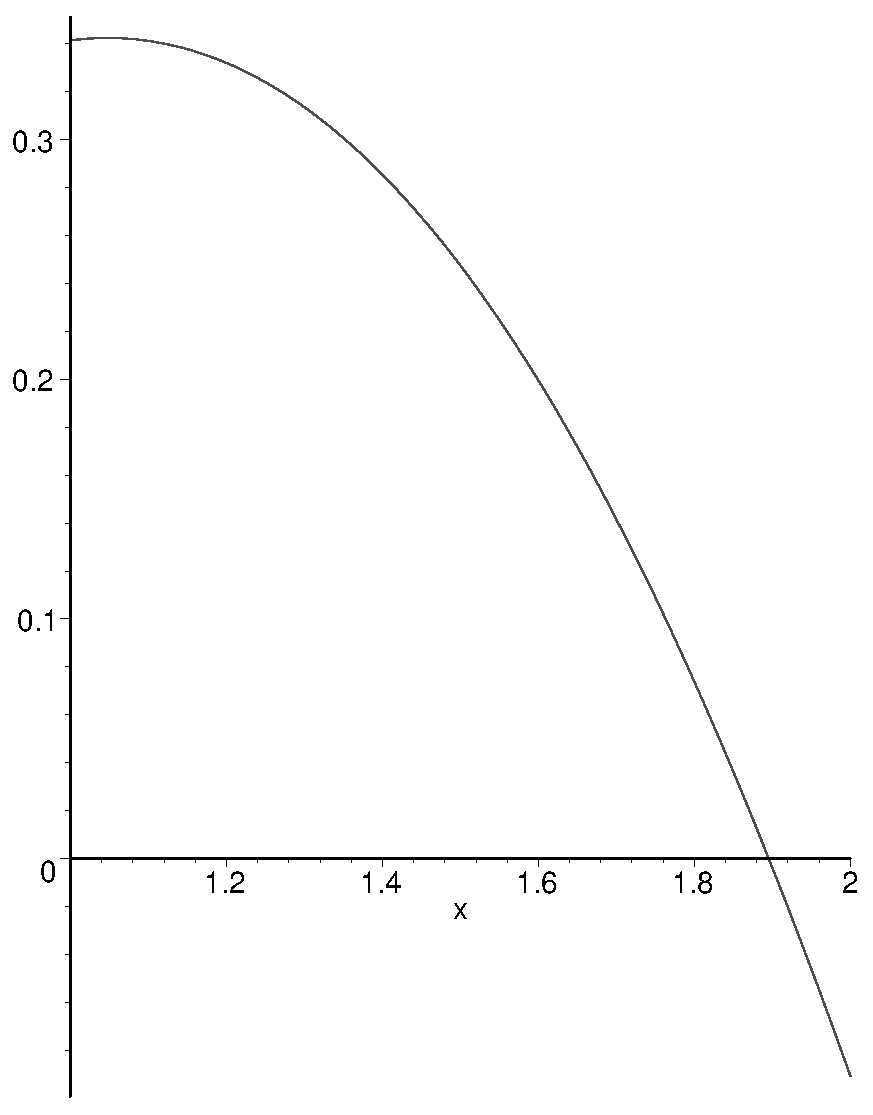
\epsfig{file=Ex46203.eps,height=4cm} \hfill
% 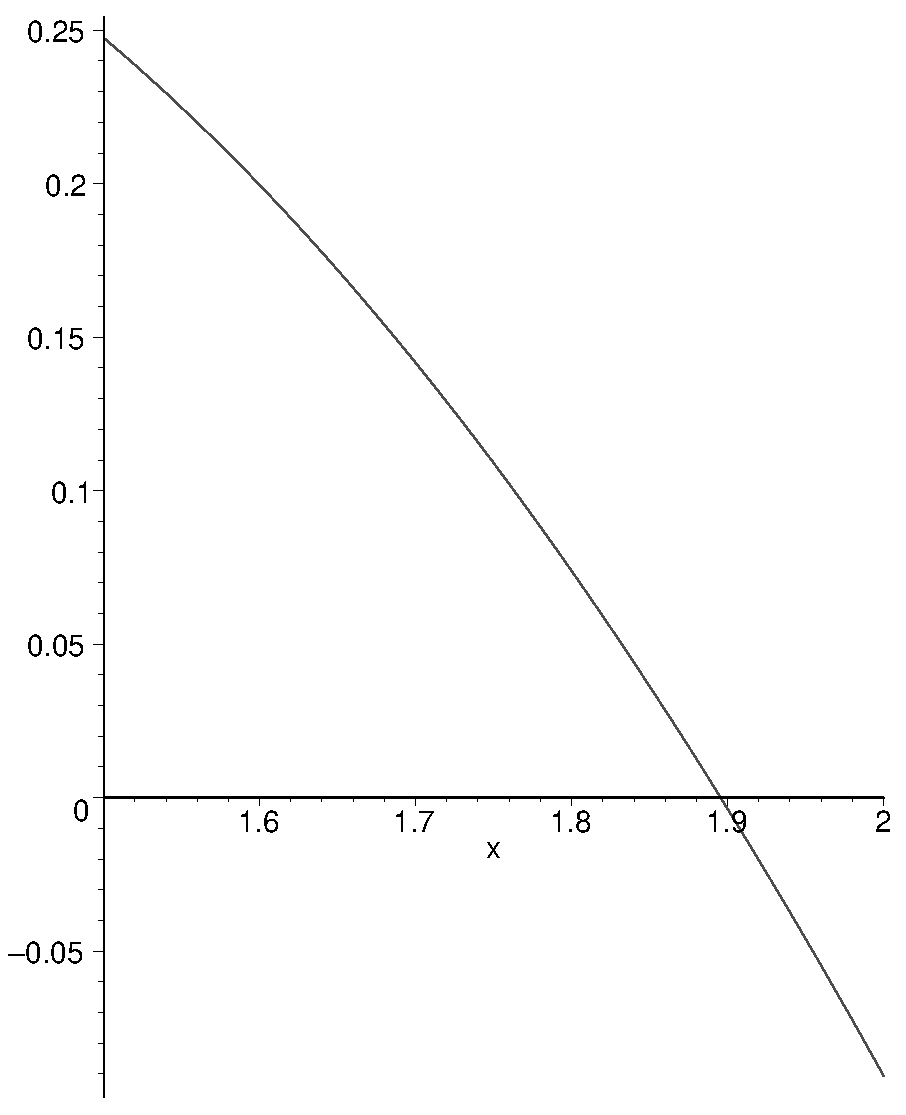
\epsfig{file=Ex46204.eps,height=4cm}
%
\includegraphics[height=4cm]{Ex46202.eps} \hfill
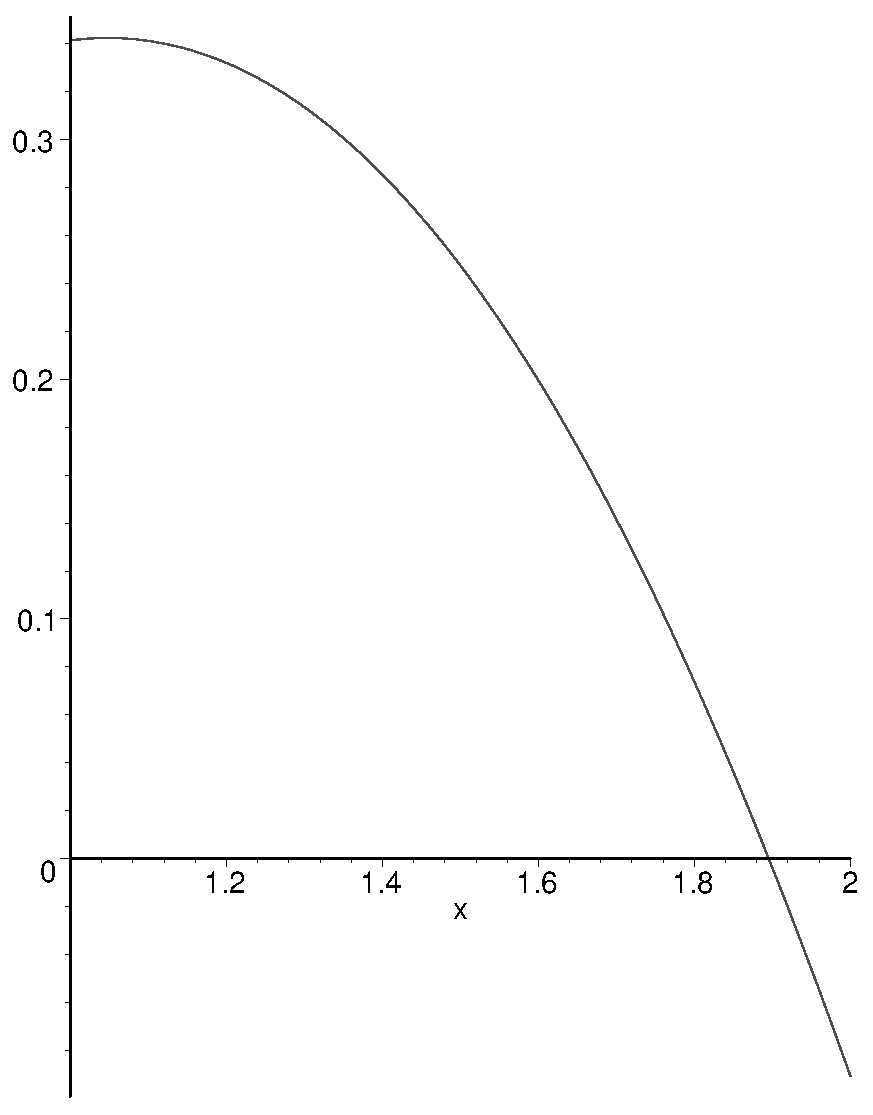
\includegraphics[height=4cm]{Ex46203.eps} \hfill
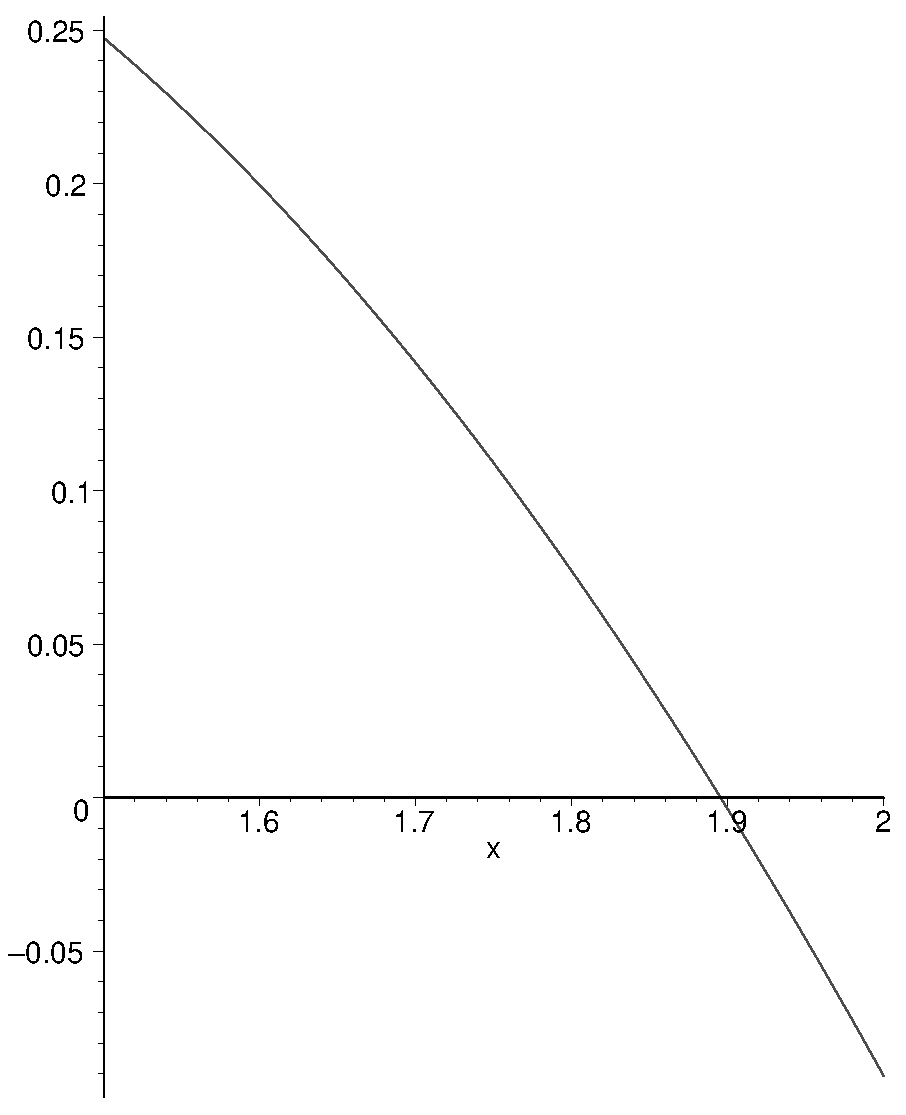
\includegraphics[height=4cm]{Ex46204.eps}
\\[0.5ex]
\underline{Numerisch:} Obiges, graphisches Verfahren kann auf ein
rein numerisches Verfahren im Computer "ubertragen werden
(der \textit{MAPLE}-Aufruf \texttt{fsolve(sin(x)=x/2,x=0.1..3}
liefert als N"aherungsergebnis $x_0 = 1.895494267$\enspace).
\bspfile{Ex462.mws}
Wir entwickeln ein Programm zur Bestimmung der Nullstelle
von $f(x) := \sin(x) - x/2$ im Intervall $[a,b]$
mittels Intervallhalbierung, wobei zur Vereinfachung
angenommen wird, da"s $f(a) >0$ und $f(b)<0$ ist.
Der Mittelpunkt des Intervalls sei mit $c:=(a+b)/2$ bezeichnet.
Dann k"onnen wir "uber die L"osung Folgendes aussagen:
$
\begin{cases}
 x_0 := c 	& \text{falls } f(c) = 0 \\
 x_0 \in [c,b]	& \text{falls } f(c) > 0 \\
 x_0 \in [a,c]	& \text{falls } f(c) < 0
\end{cases}
$\enspace.
%
Durch Redefinition der Intervallgrenzen $a$ und $b$ kann die
Nullstellensuche auf das kleinere (halbierte) Intervall
reduziert werden. Wir demonstrieren die Umsetzung mittels
eines nichtabweisenden Zyklus.
\bspfile{Ex462.cpp}

% 
% \underline{Struktogramm}: \\
% % \begin{latexonly}
% %   \special{psfile=GIF/p41a.eps.gz
% % 	   hscale=20 vscale=20
% % 	   voffset=-180
% % 	  }
% %   \vspace{6.3cm}
% % \end{latexonly}
% % \htmladdimg{p41a_4.jpg}{}
% \includegraphics[scale=0.15]{GIF/p41a.eps}
% 
% 
% Obige Bisektion kann auch mittels eines
% abweisenden Zyklus realisiert werden.\index{Bisektion}
% \\
% % \begin{latexonly}
% %   \special{psfile=GIF/p41b.eps.gz
% % 	   hscale=20 vscale=20
% % 	   voffset=-180
% % 	  }
% %   \vspace{7cm}
% % \end{latexonly}
% % \htmladdimg{p41b_4.jpg}{}
% \includegraphics[scale=0.15]{GIF/p41b.eps}
%%%%%%%%%%%%%%%%%%%%%%%%%%%%%%%%%
\begin{minipage}{0.45\textwidth}
 \underline{nichtabweisender Zyklus}: \\
 \includegraphics[scale=0.15]{GIF/p41a.eps}
\end{minipage}
\hfill
\begin{minipage}{0.45\textwidth}
 \underline{abweisender Zyklus}: \\
 \includegraphics[scale=0.15]{GIF/p41b.eps}
\end{minipage}
\\
Wir realisieren obige Bisektion als nichtabweisenden Zyklus.\index{Bisektion}
%
\includecode[linerange={7-14,19-20,45-62,67-68}]{Ex462.cpp}{Bisektion als nichtabweisender Zyklus}
%

Da Gleitkommazahlen nur mit limitierter Genauigkeit\index{Gleitkommazahl!Genauigkeit}
arbeiten, resultiert
ein Abbruchtest $f(c) = 0$ meist in einem endlosen Programm.\index{Abbruchtest}
Dem ist ein Abbruchtest wie $|f(c)| < \varepsilon$ mit einer
vorgegebenen Genauigkeit $0< \varepsilon \ll 1$ vorzuziehen.

%\enlargethispage{1ex}
\underline{Bemerkung:}
Z"ahlzyklen (\verb|for|), welche \underline{mindestens einen} Zyklus
ausf"uhren, k"onnen sowohl durch abweisende (\verb|while|)
als auch durch nichtabweisende Zyklen (\verb|do while|)
"aquivalent ausgedr"uckt werden.
Diese "Aquivalenz kann bei Verwendung der Anweisungen in \S~\ref{p:4.8}
verloren gehen.
Falls in einem Z"ahlzyklus der Abbruchtest stets \texttt{false} ergibt, d.h.
der Schleifenk"orper wird nie ausgef"uhrt, dann ist
der entsprechende abweisende Zyklus nach wie vor "aquivalent. Jedoch
ist der nichtabweisende Zyklus nicht mehr "aquivalent, da der dortige
Schleifenk"orper auch in diesem Fall einmal abgearbeitet wird.
\bspfile{Loops.cpp}
%Siehe das Beispielfile~\textit{Loops.cpp}.
%
%
%
\section{Mehrwegauswahl (\texttt{switch}-Anweisung)}
\label{p:4.7}
%
Die Mehrwegauswahl erm"oglicht ein individuelles Reagieren
auf spezielle Werte einer Variablen.
\index{Mehrwegauswahl}\index{switch!Mehrwegauswahl}

\mbox{}\hfill
\begin{minipage}[t]{0.6\textwidth}
\begin{verbatim}
switch (<ausdruck>)
 {
   case <konst_ausdruck_1> :
        <anweisung_1>
	[break;]
   ...
   case <konst_ausdruck_n> :
        <anweisung_n>
	[break;]
   default:
        <anweisung_default>
 }
\end{verbatim}
\end{minipage}
\hfill\mbox{}

\textbf{Beispiel}: Ausgabe der Zahlw"orter f"ur die ganzzahlige Eingaben
	$\{1,2,3\}$.
	%dem Intervall~$[1,3]$.
%\includecode[linerange={7-14,19-20,45-62,67-68}]{Ex470.cpp}{Demonstration der Switch-Anweisung}
\includecode[firstline=5]{Ex470.cpp}{Demonstration der Switch-Anweisung}
%

Obige \verb|switch|-Anweisung k"onnte auch mit einer
Mehrfachverzweigung (Seite~\pageref{mehrweg}) implementiert werden,
jedoch werden in der \verb|switch|-Anweisung die einzelnen Zweige
explizit "uber die  \verb|break;|-Anweisung verlassen.
Ohne \verb| break; | wird zus"atzlich der zum nachfolgenden Zweig
geh"orige Block abgearbeitet.

Es ist in C++ \emph{nicht} m"oglich, \emph{Bereiche} anzugeben, etwa der Art
\texttt{case 7..11: Anweisung; break;} anstelle der korrekten
C++-Vorgangsweise~\cite[\S1.8.4]{Breymann:2017:DCP}
% \begin{verbatim}
\\[0.5ex]
\verb| case 7: case 8: case 9: case 10: case 11:| \\
\verb|    Anweisung;| \\
\verb|    break;|
% \end{verbatim}
%
%
%
\section[Unbedingte Steuerungs"ubergabe]{Anweisungen zur unbedingten Steuerungs"ubergabe}
\label{p:4.8}
%
%\begin{itemize}
\begin{description}
 \item[\texttt{break}] Es erfolgt der sofortige Abbruch
	 der n"achst"au{\ss}eren
	 \verb|switch|, \verb|while|, \verb|do-while|, \verb|for|
	 Anweisung.\index{break}
 \item[\texttt{continue}] Abbruch des aktuellen und Start des
 	n"achsten Zyklus einer \verb|while|, \verb|do-while|, \verb|for|
	Schleife.
	\bspfile{Ex480.cpp}
 \item[\texttt{goto <marke>}] Fortsetzung des Programmes an der mit
 	\\
	\verb|<marke> : <anweisung>|
	\\
	markierten Stelle.
\end{description}
%\end{itemize}

\underline{Bemerkung :} Bis auf \verb|break| in
der \verb|switch|-Anweisung sollten obige Anweisungen
sehr sparsam (besser gar nicht) verwendet werden, da
sie dem strukturierten Programmieren zuwiderlaufen und
im Extremfall einen gef"urchteteten Spaghetticode erzeugen.
Wenn man das strukturierte Programmieren gut beherrscht, dann kann die
gezielte Verwendung von \verb|break| und \verb|continue| zu schnellerem Code
f"uhren.

\textbf{Obige Anweisungen aus \S\ref{p:4.8} sind
im Rahmen dieser LV zur L"osung von "Ubungsaufgaben und im Test nicht erlaubt.}
Einzige Ausnahme ist \verb|break| in der \verb|switch|-Anweisung.






























